\chapter{ကားရဲလ်ပရိုဂရမ် ဖီချာများ}

\section*{ကားရဲလ် ကမ္ဘာဖိုင်များ}

ကားရဲလ်ပရိုဂရမ် ဝင်းဒိုးမှာ \mytcboxinl{\fEnSnd{Load World}} ခလုတ်နှိပ်ပြီး ကမ္ဘာဖိုင်အသစ် တင်လို့ရတယ်။ ခလုတ်နှိပ်လိုက်ရင် အခုလို ဖိုင် ဒိုင်ယာလော့ဂ် ပွင့်လာမယ်။

\begin{figure}[tbh!]
\begin{tikzpicture}
    \node[anchor=south west,inner sep=0] (image) at (0,0)
        {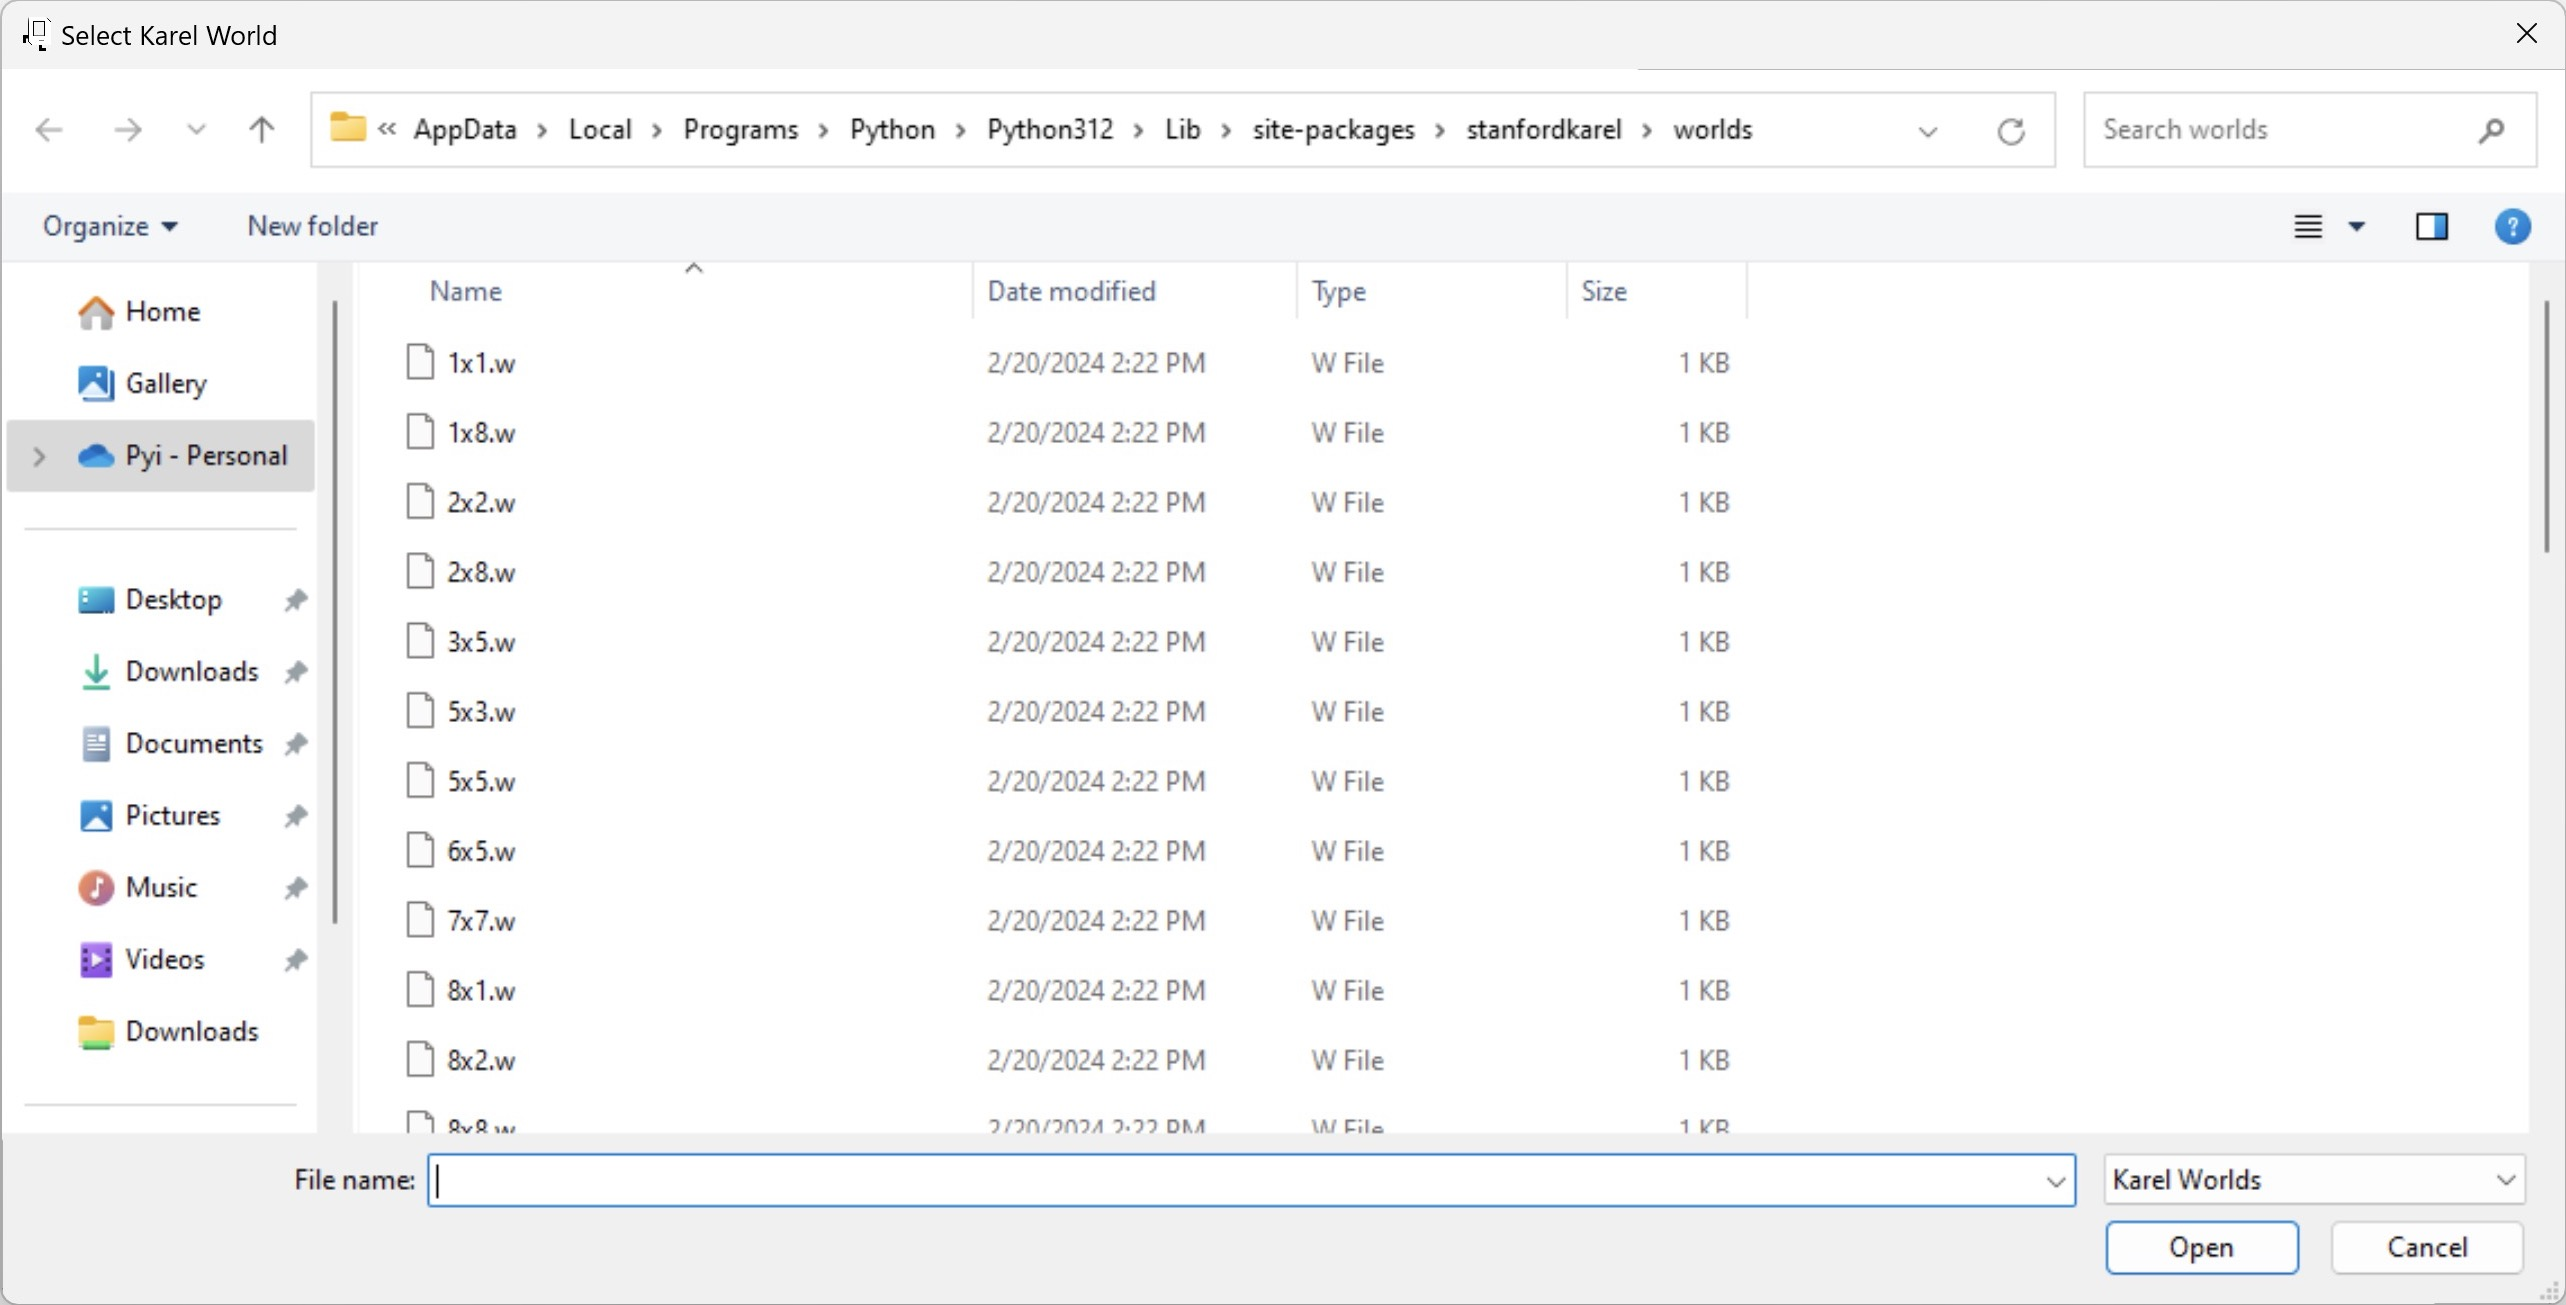
\includegraphics[width=.98\textwidth, trim={2mm 2mm 28cm 2.5mm},clip]{images/apdx02/dftworlds.jpg}};
    \drawshadow{image}
\end{tikzpicture}
\caption{} 
\label{fig:dftworlds}
\end{figure}

ဒါက \fEnSnd{stanfordkarel} လိုက်ဘရီ သူ့နဂိုအရှိအတိုင်း ပါတဲ့ \fEnSnd{worlds} ဖိုဒါပါ။ ဖိုင်တွေက  \mytcboxinl{\fEnSnd{.w}} နဲ့ ဆုံးပါတယ်။  ကမ္ဘာဖိုင်တွေကို ပင်မ ပရောဂျက်အောက် \fEnSnd{worlds} ဖိုဒါထဲမှာ ထားလို့လည်းရတယ်။ အခြားနေရာတွေမှာ ထားလို့တော့ မရဘူး။

စာအုပ်ပါ ဥပမာတွေ၊ လေ့ကျင့်ခန်းတွေအတွက် ကမ္ဘာဖိုင်တွေကို ပရောဂျက် တစ်ခုချင်းအလိုက် သီးခြား \fEnSnd{worlds} ဖိုဒါထဲမှာ ထည့်ပေးထားမှာပါ။ ပရိုဂရမ်တစ်ခုဟာ ကမ္ဘာတစ်ခုတည်းမှာပဲ အလုပ်လုပ်တာမဟုတ်ဘဲ အလားတူ ကမ္ဘာအမျိုးမျိုးအတွက် အလုပ်လုပ်အောင် ရေးပေးရတာ။ အခုပြောတာကို နားမလည်ရင် အခန်း (\fRefNo{\ref{ch:ch02}}) ဖတ်ပြီးရင် နားလည်သွားမှာပါ။

\mytcboxinl{\fEnSnd{Load World}} လုပ်တဲ့အခါ ပွင့်လာတဲ့ ဖိုင် ဒိုင်ယာလော့ဂ်က ကိုယ်လိုချင်တဲ့ \fEnSnd{worlds} ဖိုဒါ မဖြစ်နေဘူး။ သူ့နဂိုပါတဲ့ \fEnSnd{worlds} ဖိုဒါ ဖြစ်နေတယ်။ ကိုယ်ခေါ်တင်ချင်တဲ့ ဖိုင်တွေရှိတဲ့ လက်ရှိပရောဂျက်ရဲ့ \fEnSnd{worlds} ဖိုဒါကို သွားရမယ်။ ဥပမာ \fEn{PyCharm/VS Code} အတွက် \fEnSnd{MeetKarel/meet\_karel} ပရောဂျက် \fEnSnd{worlds} ဖိုဒါ လမ်းကြောင်း အပြည့်အစုံက
%
\begin{minted}[frame=lines, framerule=0pt,escapeinside=ßß]{text}
ß\fEnSnd{C:{\textbackslash}Users{\textbackslash}\textit{yourname}{\textbackslash}VSCode{\textbackslash}meet\_karel{\textbackslash}worlds}ß
ß\fEnSnd{C:{\textbackslash}Users{\textbackslash}\textit{yourname}{\textbackslash}PycharmProjects{\textbackslash}MeetKarel{\textbackslash}worlds}ß
\end{minted}
%
ဖြစ်ပါမယ်။ ဖိုင်ဒိုင်ယာလေ့ဂ်ကနေ ဖော်ပြပါ လက်ရှိပရောဂျက် \fEnSnd{worlds} ဖိုဒါကို တစ်ဆင့်ချင်း သွားပြီး တင်ချင်တဲ့ ကမ္ဘာဖိုင် (\fEnSnd{.w} ဖိုင်) ကို ရွေးရမှာပါ။

အပေါ်ကနည်းနဲ့ အဆင်မပြေခဲ့ရင် အခုလိုစမ်းကြည့်ပါ။ လက်ရှိပရောဂျက် \fEnSnd{worlds} ဖိုဒါကို ညာကလစ်နှိပ်ပြီး \fEnSnd{Copy Path} လုပ်ပါ (ပုံ \fRefNo{\ref{fig:cpwldfld}}) ။ ဖိုင် ဒိုင်ယာလော့ဂ် \mytcboxinl{\fEnSnd{File name}} မှာ ကူးထည့်ပါ (ပုံ \fRefNo{\ref{fig:pstepth}})။ \mytcboxinl{\fEnSnd{Enter}} ကီးနှိပ်ပါ။ ပရောဂျက် \fEnSnd{worlds} ဖိုဒါကိုရောက်သွားပါမယ်။ လိုတဲ့ကမ္ဘာဖိုင် ရွေးတင်ရုံပါပဲ။ ပုံ (\fRefNo{\ref{fig:prjwlds}}) မှာ \fEnSnd{meet\_karel} \fEnSnd{worlds} ကို နမူနာပြထားပါတယ်။

\begin{figure}[tbh!]
\begin{tikzpicture}
    \node[anchor=south west,inner sep=0] (image) at (0,0)
        {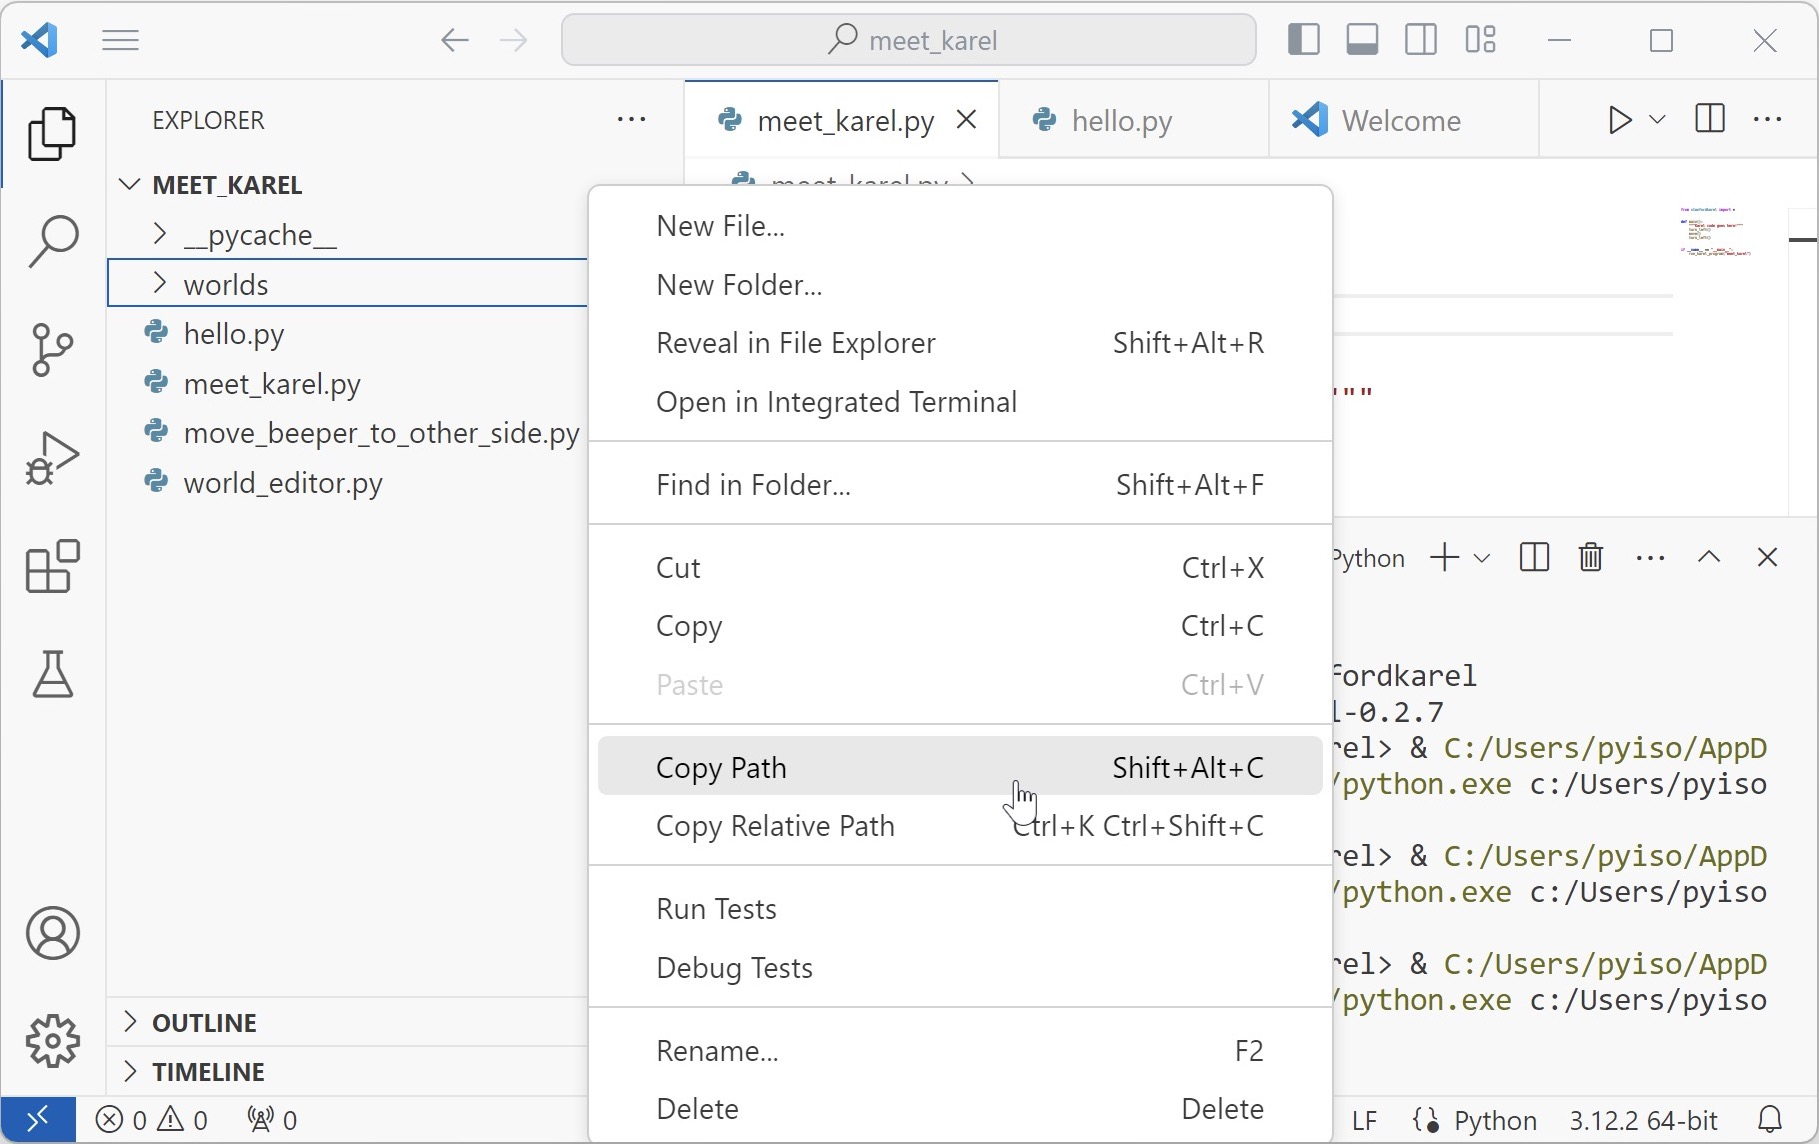
\includegraphics[width=.98\textwidth, trim={2.4mm 2mm 2mm 2mm},clip]{images/apdx02/cpwldfld.jpg}};
    \drawshadow{image}
\end{tikzpicture}
\caption{} 
\label{fig:cpwldfld}
\end{figure}

\begin{mytcbox}
အကယ်၍ အထက်ဖော်ပြပါနည်းတွေက ရှုပ်နေတယ်ထင်ရင်  မှတ်ရ/သွားရ လွယ်တဲ့ \fEnSnd{Desktop, Downloads, Documents} လို နေရာတစ်ခုခုမှာ  သီးသန့်ဖိုဒါတစ်ခု ဆောက်ပြီး ပရောဂျက်အားလုံး ထည့်ထားတာ အရှင်းဆုံးပါပဲ။ ပရောဂျက်ဖိုဒါနေရာ သိရင် ဖိုင်ဒိုင်ယာလော့ဂ်ကနေ ဘယ်လိုမဆို ရောက်အောင် သွားလို့ရပါတယ်။
\end{mytcbox}

\begin{figure}[tbh!]
\begin{tikzpicture}
    \node[anchor=south west,inner sep=0] (image) at (0,0)
        {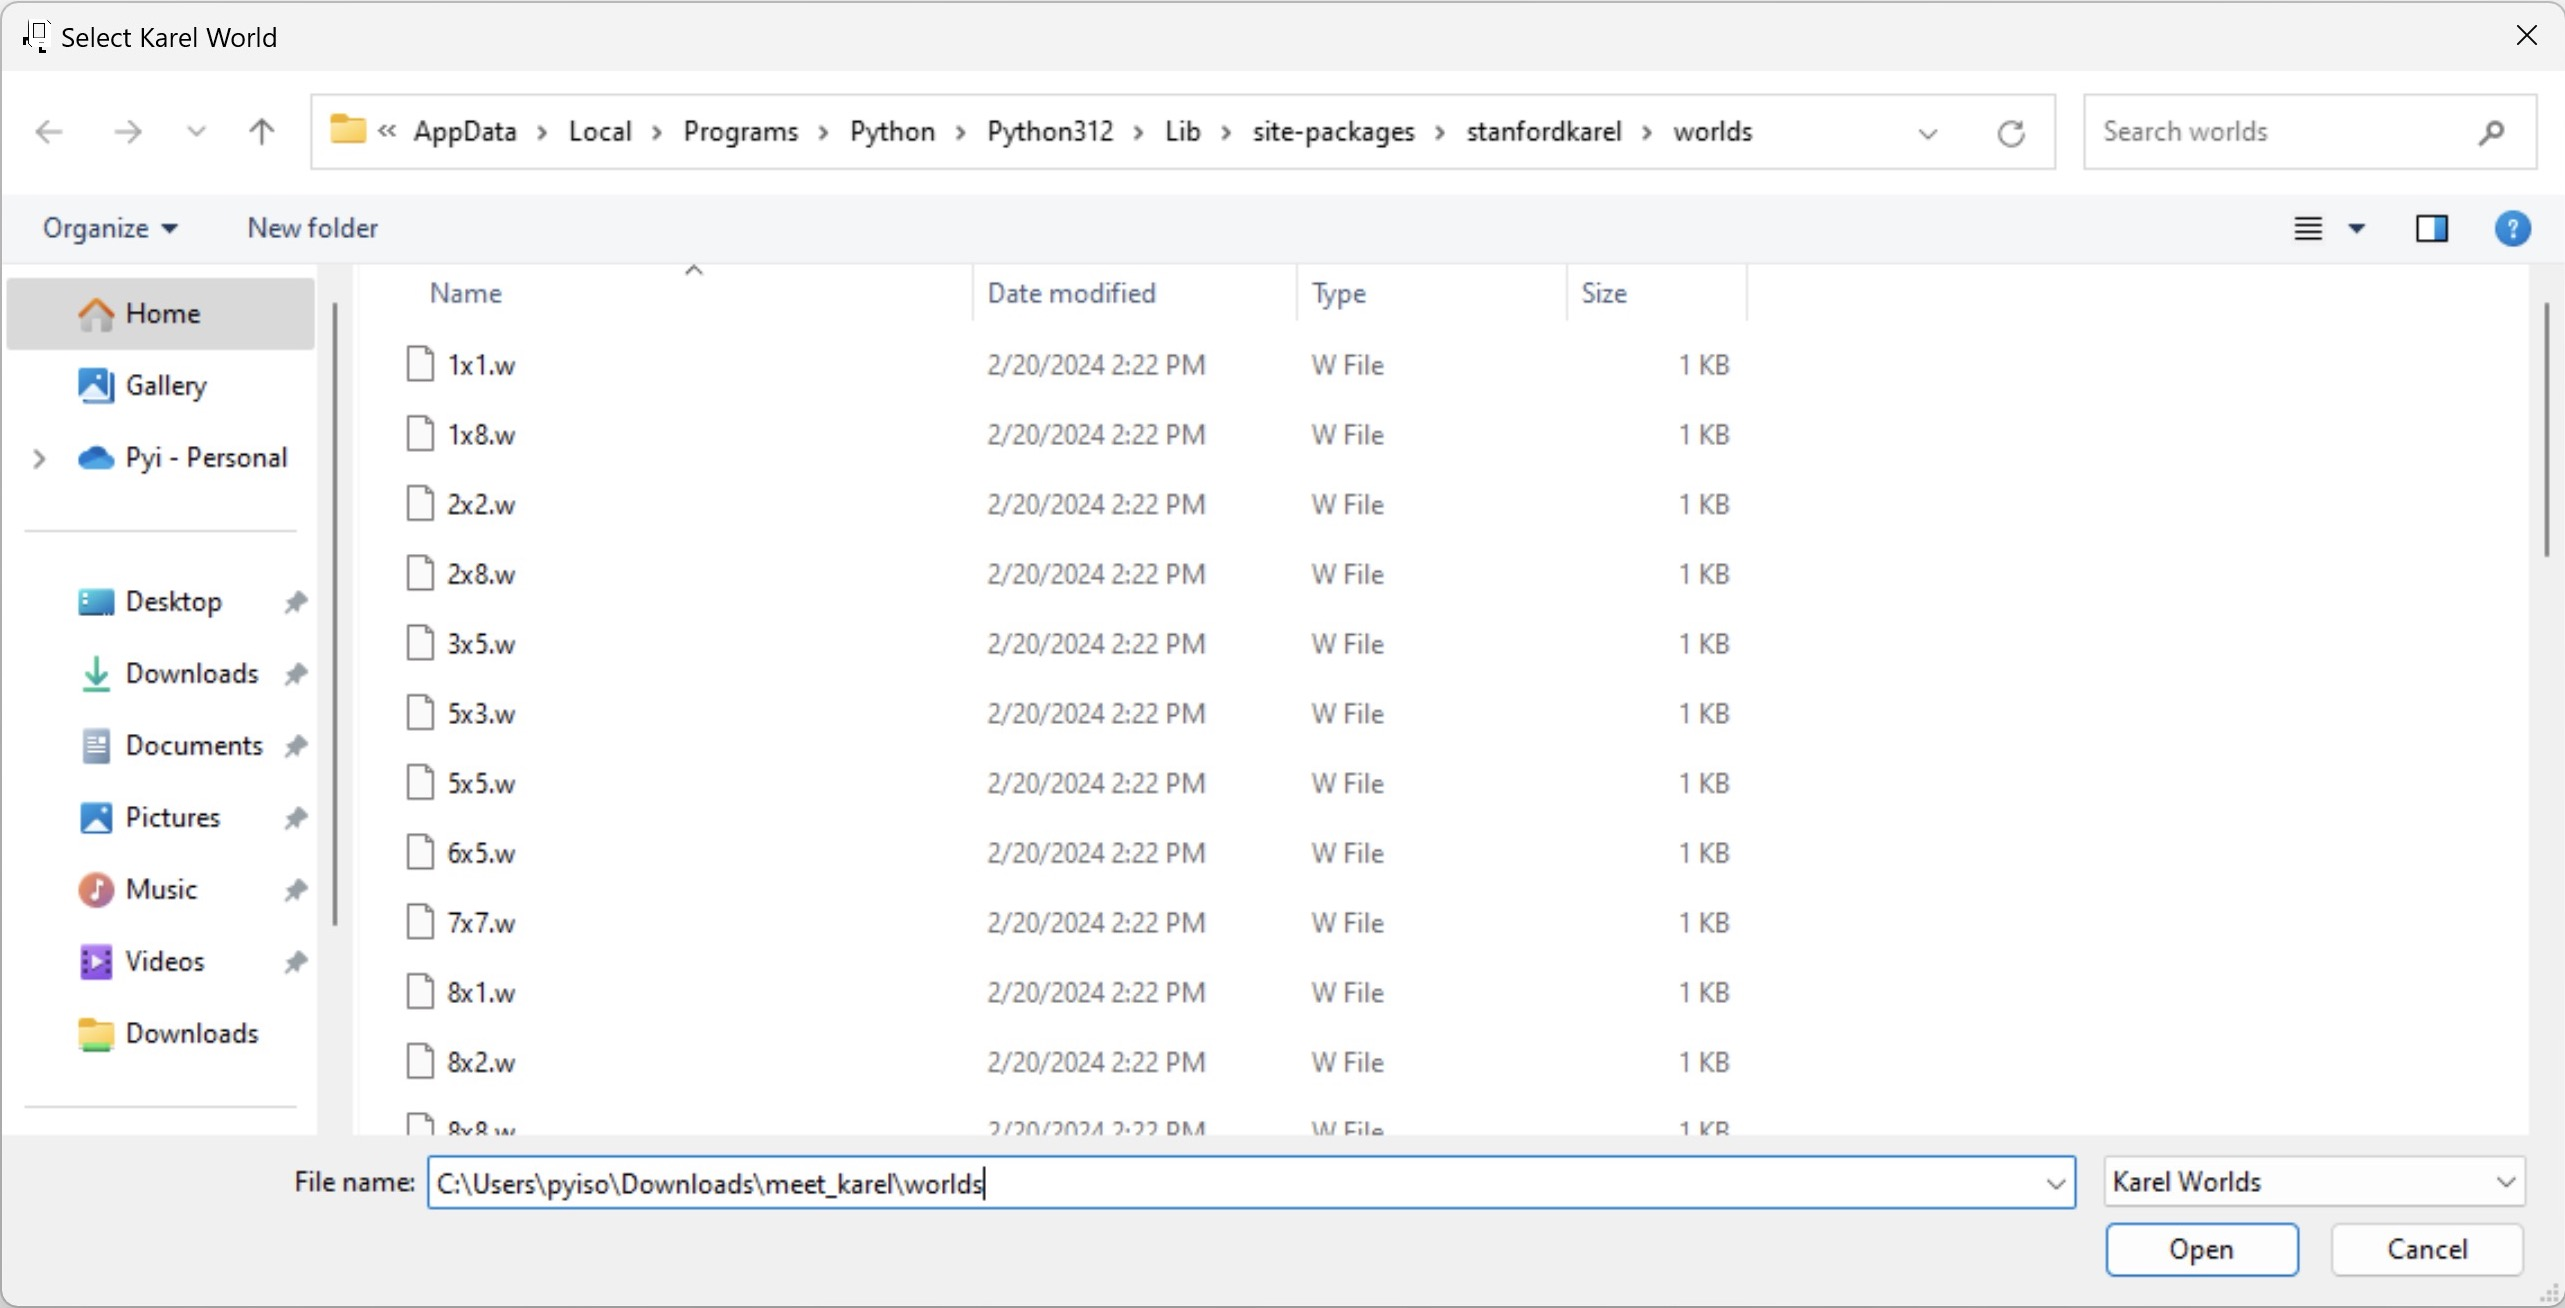
\includegraphics[width=.98\textwidth, trim={2.4mm 2mm 28cm 2mm},clip]{images/apdx02/pstepth.jpg}};
    \drawshadow{image}
\end{tikzpicture}
\caption{} 
\label{fig:pstepth}
\end{figure}

\begin{figure}[tbh!]
\begin{tikzpicture}
    \node[anchor=south west,inner sep=0] (image) at (0,0)
        {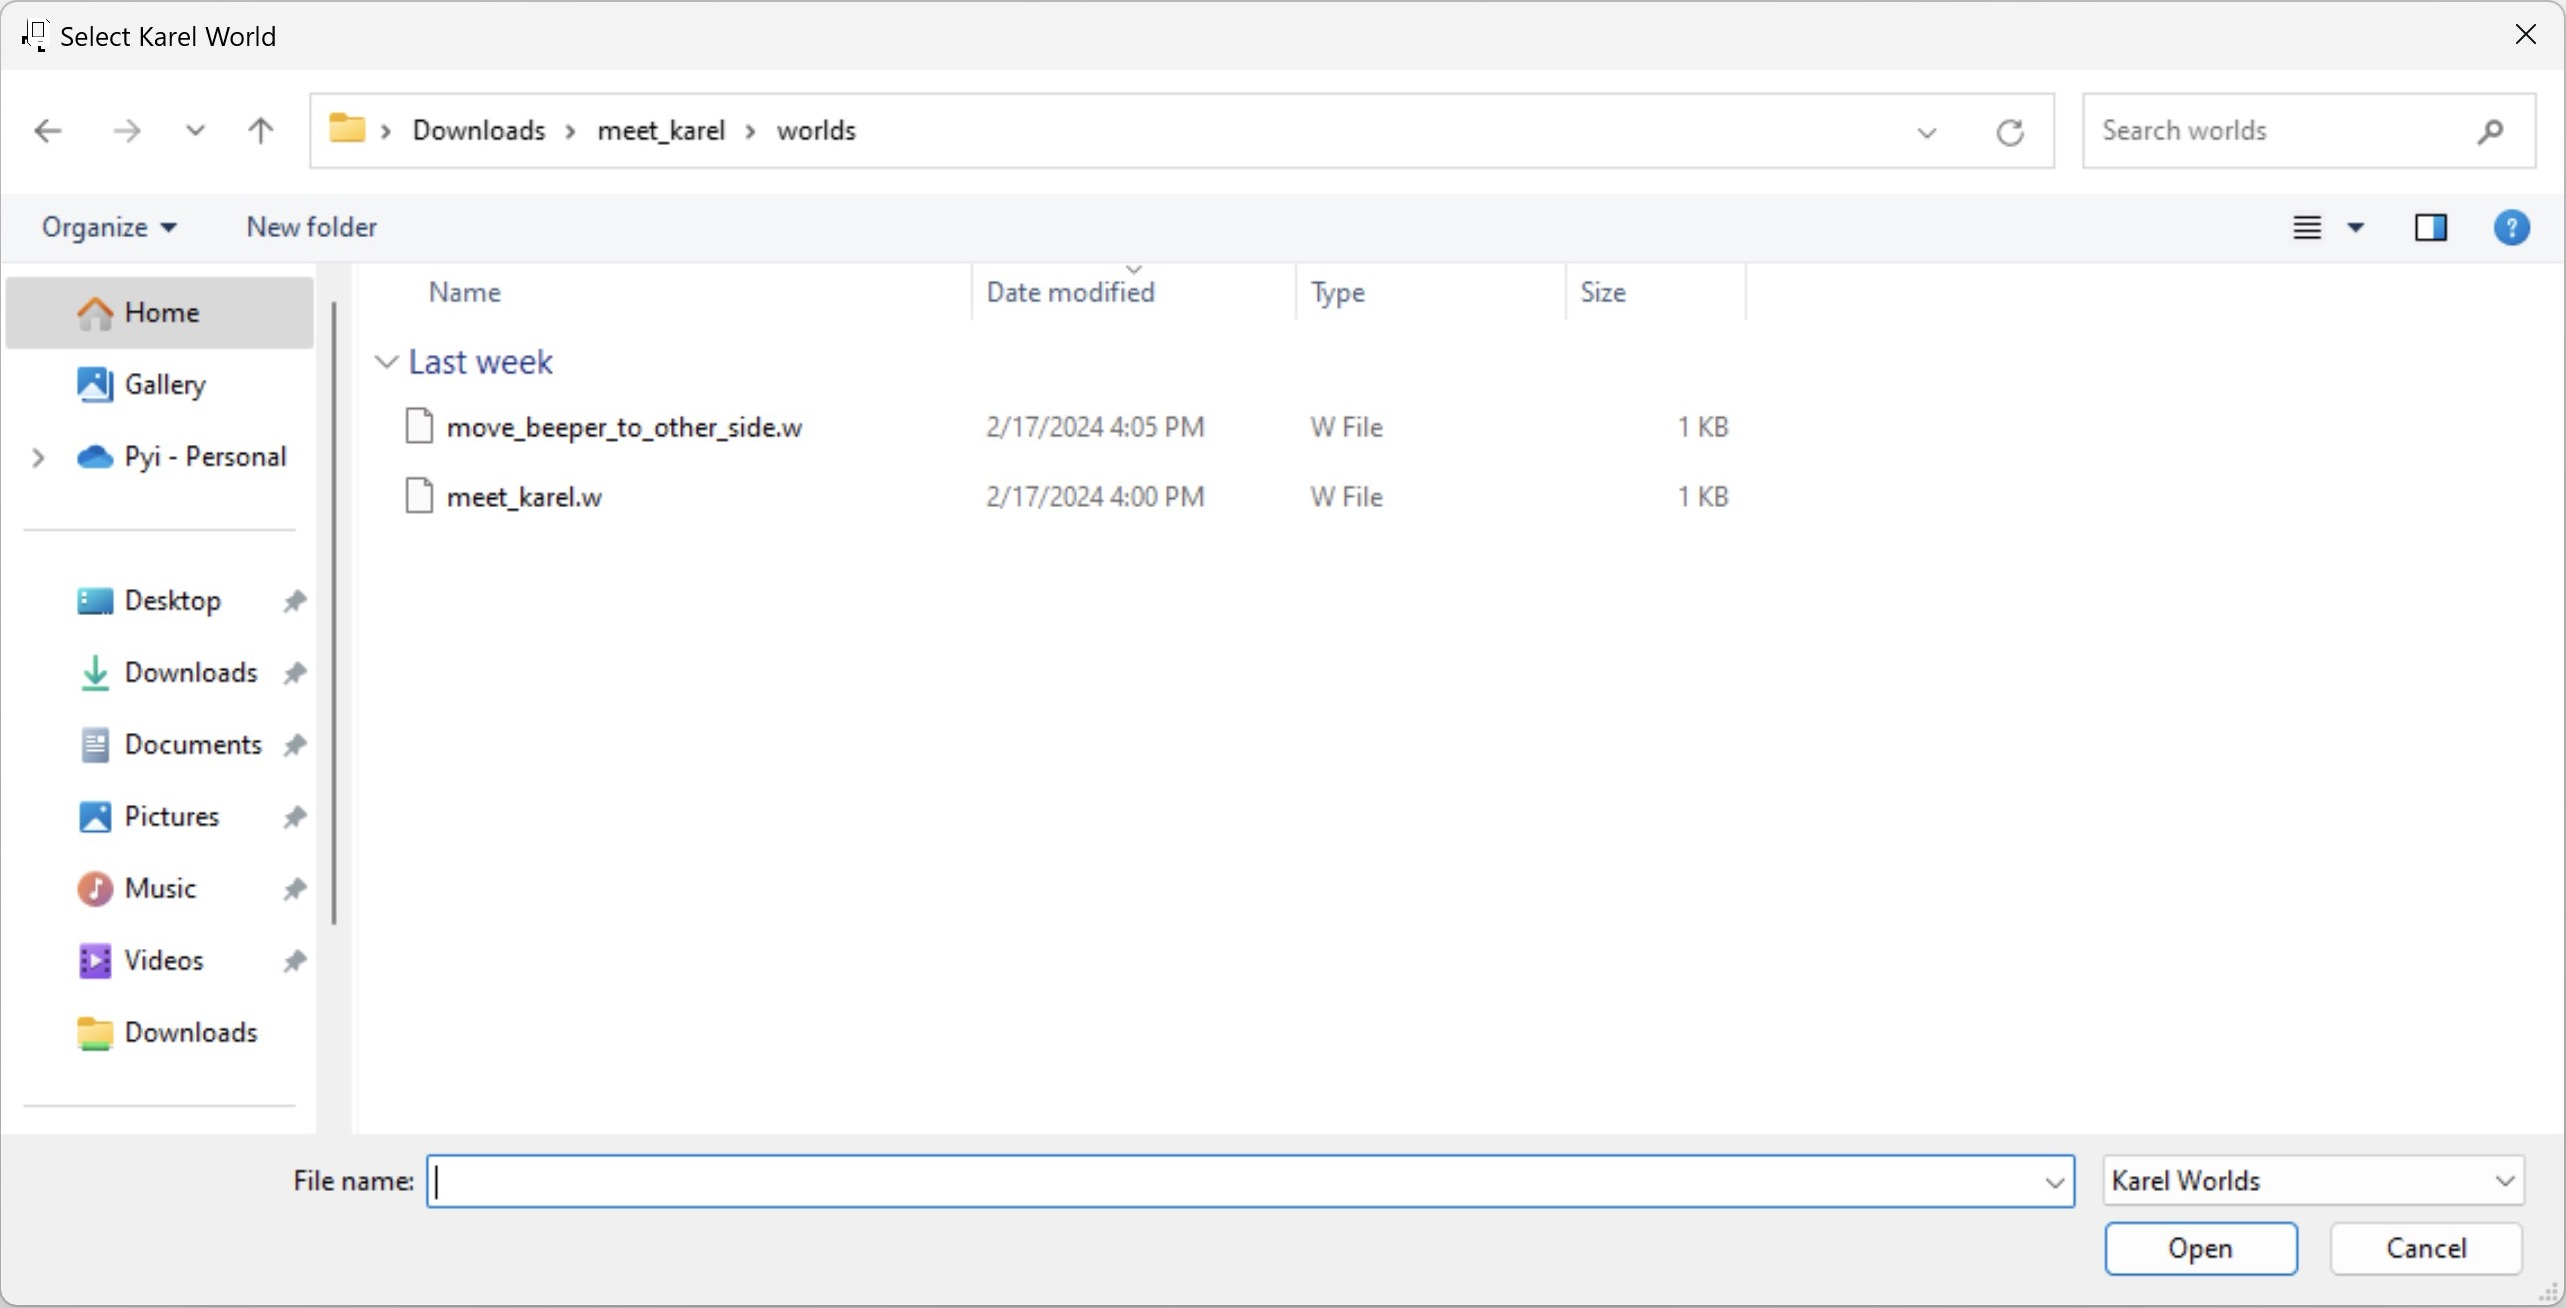
\includegraphics[width=.98\textwidth, trim={2.4mm 2mm 28cm 2mm},clip]{images/apdx02/prjwlds.jpg}};
    \drawshadow{image}
\end{tikzpicture}
\caption{} 
\label{fig:prjwlds}
\end{figure}


\clearpage

\section*{ကိုယ်ပိုင် ကားရဲလ်ကမ္ဘာ ဆောက်ခြင်း }
ကားရဲလ်ရဲ့ ကမ္ဘာ အသစ်တစ်ခုဆောက်မယ်ဆိုရင် \fEnSnd{world\_editor.py} ဖိုင်ကို ညာကလစ်နှိပ်  \fEnSnd{\mytcboxinl{Run}} ပါ။ \mytcboxinl{\fEnSnd{Would you like to load an existing world?}} လို့ ပေါ်လာပြီး \fEnSnd{Yes/No} ရွေးခိုင်ပါလိမ့်မယ်။ \fEnSnd{No} ကို နှိပ်ပါ။ ကမ္ဘာအရွယ်အစားအတွက် ကော်လံ ဘယ်နှစ်ခုလဲ၊ \fEn{row} ဘယ်နှစ်ခုလဲ ထည့်ပေးပါ။  ကိုယ်ပိုင် ကားရဲလ်ကမ္ဘာ တည်ဆောက်လို့ရတဲ့ ဝင်းဒိုးပွင့်လာပါလိမ့်မယ်။ ကားရဲလ် မျက်နှာမူရာအရပ်၊ ဘိပါအိတ်ထဲရှိ ဘိပါအရေအတွက်၊ နံရံဆောက်/ဖျက်တာ၊ ဘိပါထည့်/ဖယ်ထုတ်တာ စတာတွေ လုပ်နိုင်ပါတယ်။  \mytcboxinl{\fEnSnd{Save World}} နှိပ်ပြီး သိမ်းနိုင်ပါတယ်။ ဖိုင်ကိုသိမ်းတဲ့အခါ သူ့နဂို သိမ်းခိုင်းတဲ့ဖိုဒါ \fEn{(default world folder)} ထဲမှာ သို့မဟုတ် ပင်မ ပရောဂျက်ဖိုဒါထဲက \fEnSnd{worlds} ဖိုဒါထဲမှာ သိမ်းရပါမယ်။  

\begin{figure}[tbh!]
\begin{tikzpicture}
    \node[anchor=south west,inner sep=0] (image) at (0,0)
        {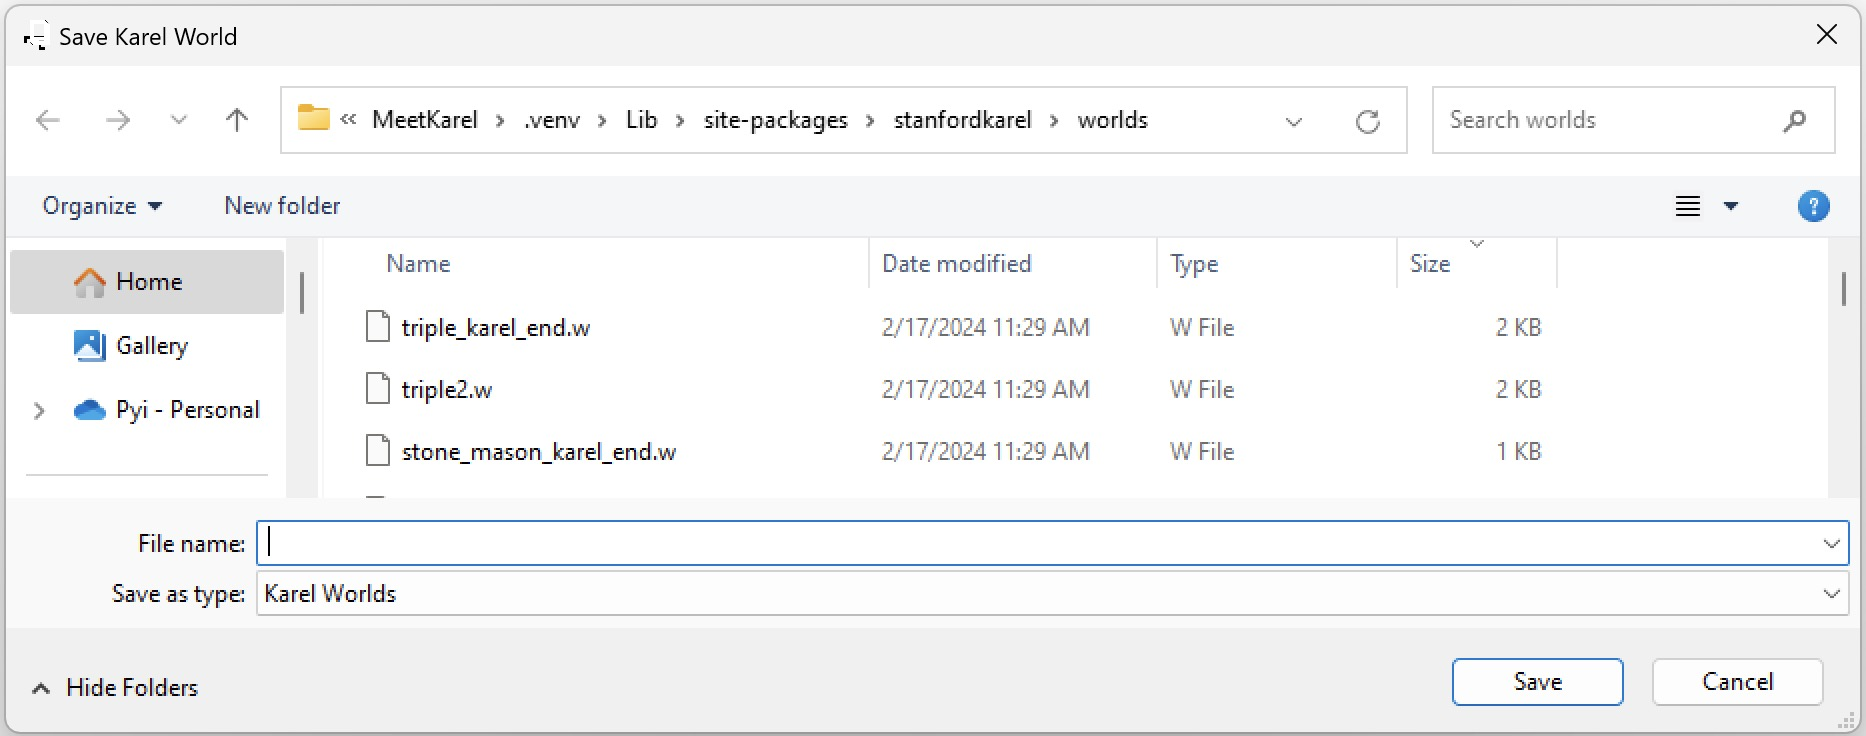
\includegraphics[width=.98\textwidth, trim={2.4mm 2cm 2mm 2mm},clip]{images/pycharm_install/default_worlds.jpg}};
    \drawshadow{image}
\end{tikzpicture}
\caption{} 
\label{fig:default_worlds}
\end{figure}

\begin{figure}[tbh!]
\begin{tikzpicture}
    \node[anchor=south west,inner sep=0] (image) at (0,0)
        {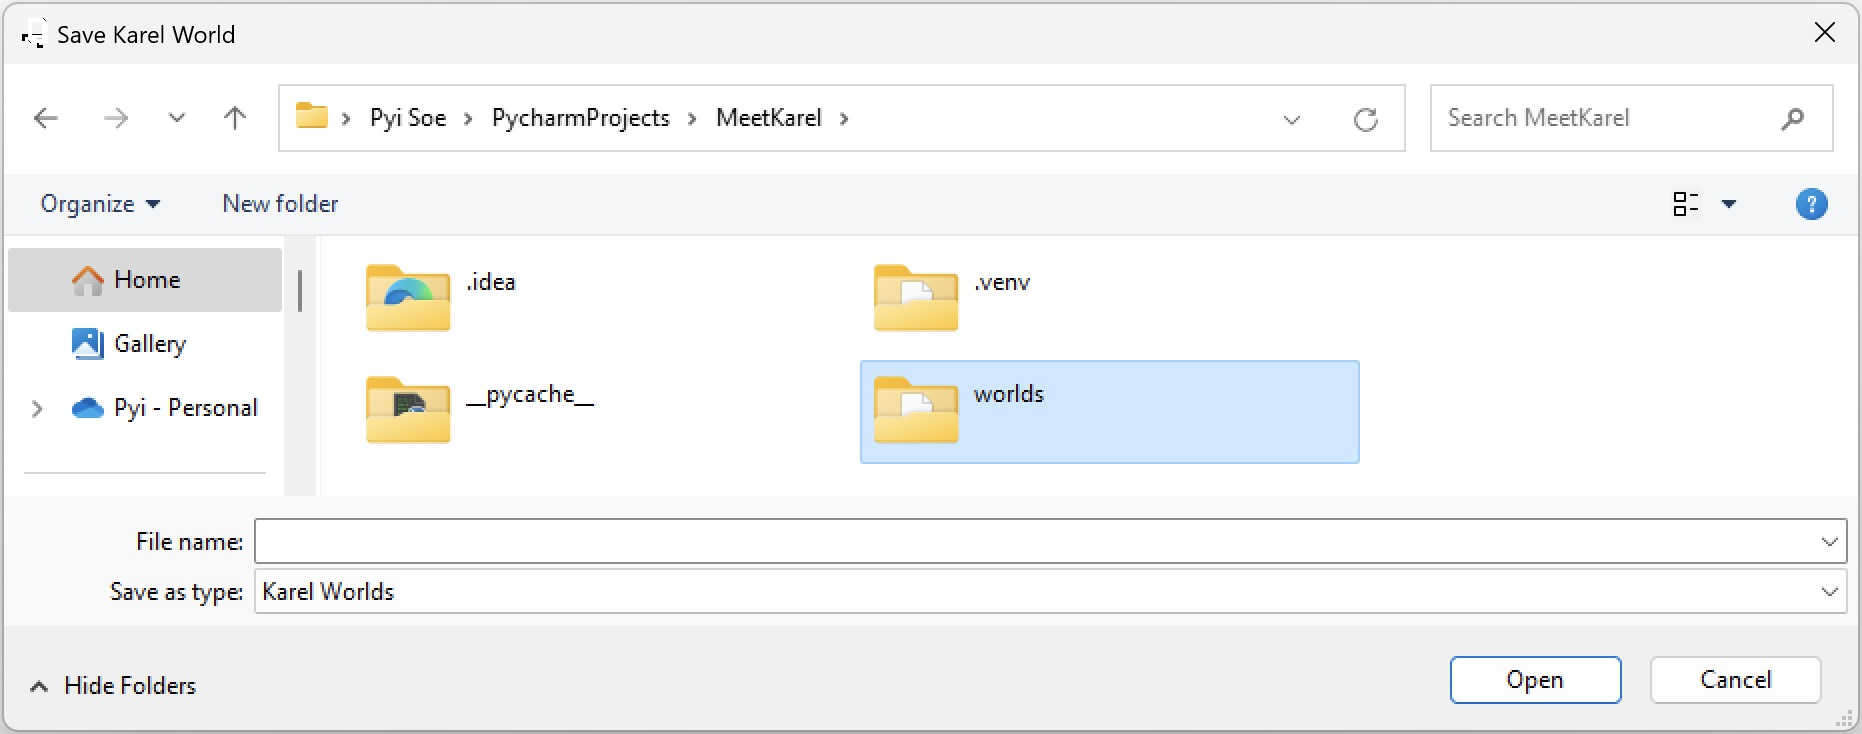
\includegraphics[width=.98\textwidth, trim={2.4mm 2cm 2mm 2mm},clip]{images/pycharm_install/proj_worlds.jpg}};
    \drawshadow{image}
\end{tikzpicture}
\caption{} 
\label{fig:proj_worlds}
\end{figure}


%\fEn{MeetKarel.zip} ကို \todo{ဒေါင်းလုဒ်လင့်ထည့်ရန်} ဒီ \fCode{https://tinyurl.com/yesz8a6j} လင့်ကနေ ဒေါင်းလုဒ်လုပ်၊ \fEn{extract} လုပ်ပြီး \fEn{lib, src, worlds} ဖိုဒါတို့ကို ပင်မ \fEn{project} ဖိုဒါအောက်မှာ ကော်ပီကူးထည့်ပါ။ \fEn{lib} ဖိုဒါကို \fEn{right click} နှိပ်ပြီး \fEn{Add as Library} လုပ်ပါ။ \fEn{src} ဖိုဒါထဲက \fEn{MeetKarel.java} ကိုဖွင့်ပြီး ပရိုဂရမ်ကို \fEn{run} ပါ။ ကားရဲလ် \fEn{Window} ပေါ်လာပါလိမ့်မယ်။ \fEn{Start Program} နှိပ်ရင် ကားရဲလ်က ဘိပါတုံးလေးကို နေရာရွှေ့ပေးပါလိမ့်မယ်။ (ပုံ \fRefNo{\ref{fig:proj_create01}} စာမျက်နှာ \fRefNo{\pageref{fig:proj_create01}} မှစ၍ \fRefNo{\ref{fig:proj_create13}} ထိ လိုအပ်ရင်ကြည့်ပါ)။ 

\clearpage


\afterpage{\blankpage}